\documentclass[11pt,letterpaper]{article}
\usepackage[lmargin=1in,rmargin=1in,tmargin=1in,bmargin=1in]{geometry}
\usepackage{../style/homework}
\usepackage{../style/commands}
\setbool{quotetype}{false} % True: Side; False: Under
\setbool{hideans}{false} % Student: True; Instructor: False

% -------------------
% Content
% -------------------
\begin{document}

\homework{9: Due 10/13}{It's fine to work on any problem, so long as it generates interesting mathematics along the way---even if you don’t solve it at the end of the day.}{Andrew Wiles}

% Problem 1
\problem{10} Suppose that you have a function $f: \mathbb{R} \to \mathbb{R}$ that is strictly increasing. 
	\begin{enumerate}[(a)]
	\item Explain why $f$ must be an injective function. 
	\item If $f$ is merely increasing, does $f$ have to be an injection? Explain why or give a counterexample. 
	\item Does $f$ have to be surjective? Explain why or give a counterexample. 
	\end{enumerate} \pspace

\sol 
\begin{enumerate}[(a)]
\item Because $f(x)$ is strictly increasing, `subsequent' values must always be larger so that no value could possibly repeat. But then $f(x)$ would be injective. To make this concrete, suppose $f(x)$ is strictly increasing but were not injective, i.e. there exist $x_1, x_2$ with $x_1 \neq x_2$ but $f(x_1)= f(x_2)$. Without loss of generality, assume $x_1 < x_2$. But then because $f(x)$ is strictly increasing, it must be that $f(x_1) < f(x_2)$, a contradiction. Therefore, it must be that $f(x)$ is injective. \pspace

\item No. For instance, if $c \in \mathbb{R}$, then $f(x)= c$ is increasing because if $x_1 < x_2$, then $c= f(x_1) \leq f(x_2)= c$. However, it is clear that $f(x)$ is not injective because $f(x)= c$ for all $x \in \mathbb{R}$. \pspace

\item Even if $f(x)$ is strictly increasing, it need not be the case that $f(x)$ is surjective. For instance, the logistic function $f(x)= \frac{5}{1 + e^{-x}}$ is clearly strictly increasing but not surjective as there is no $x$ such that $f(x)= 6$. 
	\[
	\fbox{
	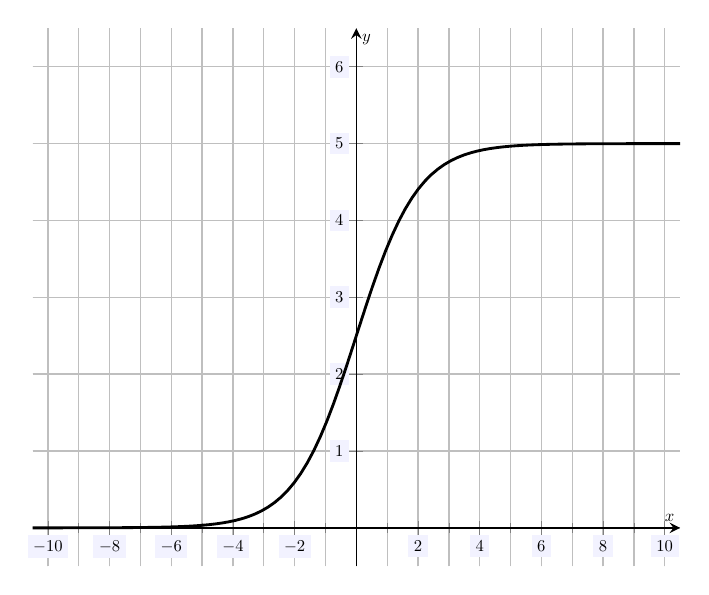
\begin{tikzpicture}[scale=1.2,every node/.style={scale=0.5}]
	\begin{axis}[
	grid=both,
	axis lines=middle,
	ticklabel style={fill=blue!5!white},
	xmin= -10.5, xmax=10.5,
	ymin= -0.5, ymax=6.5,
	xtick={-10,-8,-6,-4,-2,0,2,4,6,8,10},
	ytick={0,1,2,3,4,5,6},
	minor tick = {-10,-9,...,10},
	xlabel=\(x\),ylabel=\(y\),
	]
	\addplot[domain=-10.5:10.5,samples=100,line width=0.03cm] (x,{5/(1+exp(-x))});
	\end{axis}
	\end{tikzpicture}
	}
	\]
\end{enumerate}



\newpage



% Problem 2
\problem{10} Consider the function $f: \mathbb{R}^{\geq 2} \to \mathbb{R}$ given by $f(x)= \sqrt{x - 2}$.
	\begin{enumerate}[(a)]
	\item Solve the equation $\sqrt{x - 2}= \sqrt{y - 2}$ for $y$. 
	\item Using your work in (a), explain why this shows that $f(x)$ is injective. 
	\item Is $f(x)$ surjective? If $f(x)$ is surjective, explain why. If $f(x)$ is not surjective, find an element of the codomain not in the image of $f(x)$. 
	\end{enumerate} \pspace

\sol 
\begin{enumerate}[(a)]
\item We have\dots
	\[
	\begin{aligned}
	\sqrt{x - 2}&= \sqrt{y - 2} \\[0.3cm]
	(\sqrt{x - 2})^2&= (\sqrt{y - 2})^2 \\[0.3cm]
	x - 2&= y - 2 \\[0.3cm]
	x&= y
	\end{aligned}
	\] \pspace

\item We know a function $f(x)$ is injective if $f(x)= f(y)$ implies that $x= y$. Suppose $f(x)= \sqrt{x - 2}$. But then if $f(x)= f(y)$, we know that $\sqrt{x - 2}= \sqrt{y - 2}$. By (a), we know that this implies that $x= y$. Therefore, $f(x)$ is injective. \pspace

\item The function $f(x)= \sqrt{x - 2}$ is not surjective. For instance, $-1 \notin \im f$. Generally, if $c \in \mathbb{R}$ and $c < 0$, then $f(x) \neq c$ for all $x \in \mathbb{R}$ because $f(x) \geq 0$. 
\end{enumerate}



\newpage



% Problem 3
\problem{10} Let $A, B$ be nonempty sets. Find a bijective function from $A \times B$ to the set $B \times A$. Be sure to explain why your function is bijective. Does this mean that $A \times B$ and $B \times A$ are the same sets? Explain why or why not. \pspace

\sol It should be clear that $A \times B$ and $B \times A$ as they merely differ by a reversal of element order. We can make this rigorous: let $f: A \times B \to B \times A$ be defined by $(a, b) \mapsto (b, a)$, i.e. $f\big( (a, b) \big)= (b, a)$. It is clear that $f$ is injective: if $f\big( (a, b) \big)= f\big( (a', b') \big)$, then we have $(a, b)= f\big( (a, b) \big)= f\big( (a', b') \big)= (a', b')$. But then $(a, b)= (a', b')$, which forces $a= a'$ and $b= b'$. Therefore, $(a, b)= (a', b')$. Furthermore, given $(b, a) \in B \times A$, we know that $a \in A$, $b \in B$, so that $(a, b) \in A \times B$ and $f\big( (a, b) \big)= (b, a)$. Therefore, $f$ is surjective. But as $f$ is injective and surjective, we know that $f$ is bijective. 


\end{document}